% This document was modfied from the CVPR 2017 templates for the SBS seminar
%
% Modified by: Vitomir Struc, 6.20.2017
\documentclass[10pt,twocolumn,letterpaper]{article}
\usepackage[slovene]{babel}

\usepackage{cvpr}
\usepackage{times}
\usepackage{epsfig}
\usepackage{graphicx}
\usepackage{amsmath}
\usepackage{amssymb}
\usepackage{mathrsfs}
\usepackage{amsfonts}

% Include other packages here, before hyperref.

% If you comment hyperref and then uncomment it, you should delete
% egpaper.aux before re-running latex.  (Or just hit 'q' on the first latex
% run, let it finish, and you should be clear).
\usepackage[breaklinks=true,bookmarks=false]{hyperref}

\cvprfinalcopy % *** Uncomment this line for the final submission
\def\cvprPaperID{1} % 
\def\httilde{\mbox{\tt\raisebox{-.5ex}{\symbol{126}}}}

% Pages are numbered in submission mode, and unnumbered in camera-ready
\ifcvprfinal\pagestyle{empty}\fi
\setcounter{page}{4321}
\begin{document}

%%%%%%%%% TITLE
\title{Večmodalna detekcija ovir na vodni površini}

\author{Autor: Tilen Tinta, Mentor: izr. prof. dr. Janez Perš, as. dr. Jon Muhovič\\
{\tt\small Univerza v Ljubljani, Fakulteta za elektrotehniko} \\
{\tt\small tt5935@student.uni-lj.si, janez.pers@fe.uni-lj.si, jon.muhovic@fe.uni-lj.si}
% For a paper whose authors are all at the same institution,
% omit the following lines up until the closing ``}''.
% Additional authors and addresses can be added with ``\and'',
% just like the second author.
% To save space, use either the email address or home page, not both
}

\maketitle
%\thispagestyle{empty}

%-------------------------------------------------------------------------

%%%%%%%%% ABSTRACT
\begin{abstract}
   V zadnjih letih lahko zasledimo vedno več govora o avtonomni vožnji. Največ razvoja je ta doživela v avtomobilski industriji, a to ne pomeni, da se ta ne razvija tudi drugje. Eno takih je na primer pomorstvo oziroma ladijski promet. Detekcija ovir na vodnih površinah prinaša nove in drugačne izzive v primerjavi z detekcijo na kopnem. Enako velja tudi za podatkovne zbirke. Te so za kopenski promet že dobro razvite in dodelane, kar pa za zbirke namenjene vodnemu prometu še ne velja. V tem članku predstavljamo nekaj pristopov k več modalni detekciji in segmentaciji, ki temeljijo na različnih metodah in vhodnih podatkih za dosego zastavljenih ciljev. Prvi dve metodi uporabljata arhitekturo SegFormer in sta namenjeni semantični segmentaciji barvnih ter termalnih slik. Drugi dve metodi pa temeljita na modelu YOLO11 in omogočata detekcijo ovir na vodni gladini, pri čemer prav tako uporabljata obe kategoriji slik kot vhodne podatke. Na področju segmentacije smo izvedli primerjavo med SegFormer-jem in klasičnim U-Net-om, pri čemer rezultati kažejo, da pri razpoložljivi količini podatkov oz. z uporabo le osnovne zbirke podatkov SegFormer ne dosega bistvene prednosti. Podobno smo analizirali rezultate istih arhitektur z različnimi vhodnimi oblikami podatkov za detekcijo ovir. Izkazalo se je, da so za dnevno plovbo na kateri so bili učni podatki tudi pridobljeni barvne slike precej bolj primerne od termalnih.
\end{abstract}

%%%%%%%%% BODY TEXT
\section{Uvod}

Avtonomna vožnja je področje, ki v zadnjem času doživlja velik razvoj. Največ govora o njej je predvsem v cestnem prometu. Ta pa ni prisotna le v avtomobilski industriji. Raziskave in prve implementacije se pojavljajo tudi v pomorstvu, kjer se avtonomna plovba srečuje z drugačnimi izzivi zaradi spremenljivih okolij značilnih za pomorstvo.

Detekcija ovir na vodi je poseben problem, ki se razlikuje od detekciji na kopnem. Vodna površina se stalno spreminja zaradi vplivov okolja, kot je na primer valovanje, bleščanje, odsevi in na vodi velikokrat tudi megla. Poleg tega je razvoj podatkovnih zbirk za ta namen še v zgodnji fazi. Zaradi tega je učenje robustnih modelov strojnega učenja veliko težje za razliko od cestnega prometa, kjer so podatkovne zbirke dobro anotirane in je teh veliko.

V tem članku predstavimo več pristopov za zaznavanje in segmentacijo ovir na vodni gladini z uporabo različnih vhodnih oblik podatkov. Osredotočamo se na uporabo barvnih in termalnih slik ločeno, zajetih z dvema neodvisnima kamerama. V prvem delu predstavljamo semantični segmentaciji z uporabo arhitekture SegFormer, kjer rezultate primerjamo s klasičnim U-Net modelom. V drugem delu pa se osredotočimo na detekcijo ovir s pomočjo modela YOLO11, prilagojenega za delo z enim razredom, ki predstavlja dinamične ovire.

Skozi analizo različnih arhitektur in vhodnih podatkov raziskujemo, kako vrsta vhodnih podatkov vpliva na natančnost zaznave. Pokazali bomo, da barvne slike pri dnevnih pogojih prekašajo termalne, zlasti na področju detekcije premikajočih se ovir. Naše ugotovitve podajajo prednosti in omejitve posameznih pristopov pri segmentaciji in detekciji ovir na vodi. 
%-------------------------------------------------------------------------

\begin{figure}[t]
    \centering % Središčenje slike
    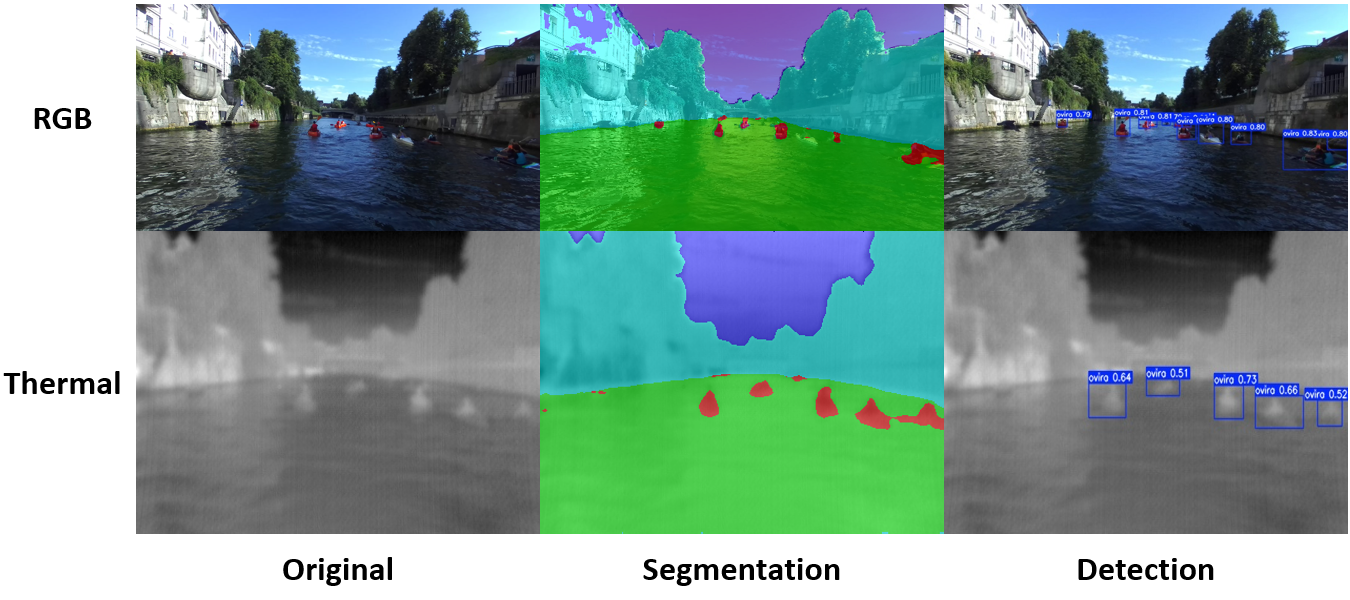
\includegraphics[width=0.5\textwidth]{Slike/teaser.PNG} % Vstavljanje slike
    \caption{Primeri segmentacije in detekcije na različnih modalitetah} % Napisan napis
    \label{fig:teasere_slika} % Oznaka za referenciranje slike
\end{figure}

%%%%%%%%% SORODNA DELA
\section{Sorodna dela}

Prvi poskusi zaznave ovir na vodi so temeljili na statistični segmentaciji, vizualni pozornosti in stereoskopskem vidu, vendar so se ti izkazali za nezanesljive v nekaterih pogojih, kot so odsevi ali zrcaljenja \cite{Cane2016CVPRW, Prasad2019Background, Wang2013ROBIO, Cane2019AVSS}. Z uporabo globokih nevronskih mrež, kot sta Faster R-CNN in YOLO, so dosegli velik napredek, vendar splošni modeli, naučeni na kopenskih podatkih, v pomorstvu pogosto niso zanesljivi, še posebej za zaznavanje manjših in dinamičnih objektov \cite{Bochkovskiy2020YOLOv4, Steccanella2020RAS, Cane2019AVSS}.

Da bi dosegali boljše rezultate kot klasični detektorji, so bili razviti segmentacijski pristopi, ki sliko razdelijo na plovne in neplovne dele. Kristan et al. so predlagali takšen način obravnave slike, ki omogoča zaznavo dinamičnih in statičnih ovir hkrati \cite{Kristan2016Cyber}. Metode, kot so WaSR, WODIS in ShorelineNet, so posebej prilagojene za pomorsko segmentacijo in učinkovito odpravljajo motnje, kot so odsevi na vodi ali slaba vidljivost \cite{Bovcon2021Tcyb, Chen2021TIM, Yao2021IROS}. V zadnjem času se uveljavljajo tudi panoptični modeli, ki poleg semantične segmentacije omogočajo tudi detekcijo in kategorizacijo ovir ob istem času. Ena od podatkovnih zbirk s katero se to lahko preizkuša je LaRS \cite{Zust2023ICCV}.

Velik izziv pri zaznavanju ovir na vodi so omejitve posameznega senzorja, zato je mogoče zaslediti tudi uporabo večmodalnih pristopov. Ti običajno združujejo podatke iz barvnih in termalnih kamer ter drugih senzorjev kot so LiDAR, radar itd., kar poveča robustnost sistema \cite{BenShoushan2023RS}. Kombinacija RGB in IR slik je pokazala prednosti predvsem kjer je prisotno bleščanje oz. ponoči, medtem ko termalne slike omogočajo detekcijo tudi v slabši vidljivosti npr. megli \cite{BenShoushan2023RS, Kristo2020Access}.

V zadnjih letih prevladujejo ti. enostopenjski detektorji, kot so različice YOLO, ki omogočajo realnočasovno obdelavo in so tako postali skoraj da standard v avtonomni vožnji\cite{Bochkovskiy2020YOLOv4}. Poleg konvolucijskih mrež se vse bolj uveljavljajo arhitekture, ki temeljijo na transformerjih, npr. DETR in DINO, ki omogočajo učinkovito učenje kompleksnih vzorcev in povezave med deli slik \cite{Carion2020DETR, Zhang2023DINO}. Na področju segmentacije sta se uveljavila SegFormer in Mask2Former, ki izkoriščata prednosti transformerjev za natančno in učinkovito segmentacijo \cite{Xie2021SegFormer, Cheng2022Mask2Former}. Sodobni sistemi povezujejo podatke iz različnih virov oz. modalitet in uporabljajo  mehanizme pozornosti za doseganje še boljše zaznave v zahtevnih okoljih kot je pomorstvo \cite{Cheng2021RAL}.

%-------------------------------------------------------------------------

%%%%%%%%% METODOLOGIJA DEL
\section{Metodologija}
V tem poglavju predstavljamo naš pristop k statičnih segmentaciji in detekciji dinamičnih ovir na vodni površini. Osrednji cilj je preveriti ustreznost izbranih modelov za tovrstne naloge ob uporabi različnih vhodnih podatkovnih modalitet ter oceniti natančnost rezultatov, ki jih ti modeli omogočajo.

\subsection{Podatkovna zbirka}
Kot že omenjeno, podatkovna zbirka vsebuje dve podatkovni modaliteti. To so slike zajete s senzorskim sistemom razvitim na Fakulteti za elektrotehniko univerze v Ljubljani v laboratoriju za strojno inteligenco, ki je bil nameščen na ladji. Zajem slik je potekal podnevi med plovbo po reki Ljubljanici, v realnih pogojih plovbe. Prva modaliteta slik so klasične barvne slike zajete z ZED kamero resolucije 2208x1242 in 24 bitno barvno globino. Druga modaliteta so termalne slike zajete s termovizijsko kamero Device-ALab SmartIR384L z resolucijo 384x288 z 16 bitno barvno globino. Vse slike so bile ročno anotirane za namen učenja semantične segmentacije. Anotacije vključujejo sedem razredov: statične ovire, dinamične ovire, voda, nebo, luknje v vodi, zavržena območja in deli ladje, s katero so bile slike zajete. Ker nas v tej raziskavi zanimajo le štiri kategorije torej statične in dinamične ovire, voda ter nebo so bile ostale oznake zavržene oz. uvrščene pod drug razred. Drugi del zbirke namenjen detekciji je ravno tako sestavljen iz obeh modalitet. Podatki o detekciji dinamičnih objektov na slikah so zapisani v formatu \texttt{json} v obliki, ki tvori okvir okrog objekta. 

Vseh barvnih slik v bazi je 580, katere so bile deljene na učno množico z 391, validacijsko z 98 in testno z 91 slikami. Enako je bilo storjeno tudi z termalnimi slikami, le da so zaradi manjkajočih slik bile množice manjše. V tem primeru je učno množico sestavljalo 337, validacijsko 88 in testno ravno tako 88 slik, torej skupaj 513 slik.

Uporabljene so bile vse slike, te ki sestavljajo učno in validacijsko množico pa so bile v postopkih učenja tudi augmentirane. Vseh slik ni bilo ravno veliko, kar je kasneje tudi razvidno iz rezultatov učenja nevronskih mrež. 

\subsection{U-Net}
U-Net je ena od najbolj uveljavljenih arhitektur za nalogo semantične segmentacije. V osnovi je bila razvita za medicinske slike \cite{ronneberger2015unetconvolutionalnetworksbiomedical}. Ključna značilnost U-Net-a je njegova simetrična struktura, ki je sestavljen iz dveh delov. Prvi ali vhodni del pripada enkoderju, drug del pa dekoder. Enkoder postopoma zmanjšuje dimenzije vhodne slike in tako povečuje zgoščenost podatkov z  konvolucijami in združevanjem (angl. pulling). 
Dekoder postopoma rekonstruira prostorsko ločljivost segmentirane maske. To izvaja z uporabo dekonvolucije (angl. up-convolution). Da ta doseže ustrezno resolucijo uporablja posebne povezave (angl. skip connections) med ustreznimi nivoji encoderja in dekoderja. 

U-Net je še posebej primeren za primere, kjer je na voljo manjša količina podatkov. Zaradi svoje strukture in lokalnih konvolucij se mreža dobro generalizira tudi z malo učnimi primeri. V našem primeru je uporaba U-Neta smiselna, ker podatkovna zbirka vsebuje malo slik, poleg tega pa vsebuje značilnosti, kot so majhni objekti na primer dinamične ovire, ki zahtevajo natančno segmentacijo.\cite{futrega2021optimizedunetbraintumor}

V naši implementaciji smo uporabili različici U-Neta, prilagojeno za delo z barvnimi slikami ter termalnimi slikami. Razlika med njima je bila le v nalagalniku vhodnih podatkov.

Rezultati modela U-Net so služili kot primerjalna osnova za ocenjevanje učinkovitosti sodobnejših arhitektur, kot je SegFormer, ki uporablja transformerje za bolj globalno obravnavo slike.

\begin{figure*}[t] % [t] postavi sliko na vrh strani
    \centering
    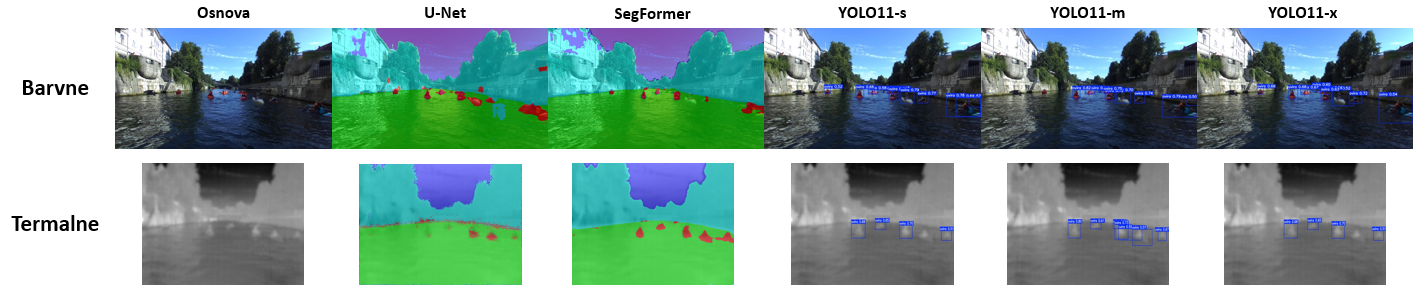
\includegraphics[width=\textwidth]{Slike/teaser2.PNG} % prilagodite širino na celotno stran
    \caption{Primeri izhodnih slik posameznih modelov glede na enake vhodne slike}
    \label{fig:prikaz_modelov_velikaSlika} % oznaka za referenciranje
\end{figure*}

\subsection{SegFormer}

SegFormer je ena od novejših arhitektur za semantično segmentacijo, ki temelji na uporabi transformerjev. Model združuje princip postopnega pridobivanja značilk z uporabo gradnikov transformerjev in preprostega segmentacijskega dela brez potrebe po pozicijskem kodiranju kot ga najdemo pri slikovnem transformetju (angl. vision transformer - ViT)\cite{dosovitskiy2021imageworth16x16words}.

Glavni del modela predstavlja encoder, ki uporablja hierarhično strukturo transformer blokov za obdelavo slike na različnih resolucijah. Za razliko od klasičnega CNN-ja SegFormer namesto konvolucijskih slojev uporablja efektivne samopozornostne mehanizme (angl. efficient self-attention). Ti omogočajo boljše zajemanje konteksta na celotni sliki in logične povezave med oddaljenimi deli slike. Ta pristop se je izkazal kot zelo efektiven pri segmentaciji kompleksnejših slik, kjer so pomembne tako lokalne kot globalne značilnosti.

Decoder oz. segmentacijski del je zasnovan kot preprost večslojni perceptron (angl. multi layer perceptron - MLP), ki na podlagi značilk iz vseh nivojev encoderja združi informacije in izdela končno segmentacijsko masko. Zaradi svoje preprostosti omogoča hitro inferenco in manjše število parametrov. To naredi model primeren tudi za uporabo na napravah z omejeno računsko močjo.

Posebnost SegFormerja je tudi v tem, da ne uporablja ne absolutnega in ne relativnega pozicijskega kodiranja. Namesto tega se model povezave med deli slike uči prek prekrivajočih se konvolucijskih vzorcev (angl. overlapping patch embedding).
To izboljša sposobnost generalizacije vhodnih podatkov različnih velikosti \cite{xie2021segformersimpleefficientdesign}.

\subsection{YOLO11}

YOLO11 je v času pisanja najnovejša različica v seriji modelov YOLO (angl. You Only Look Once). Spada med modele z tako imenovano enojno obdelavo slike (angl. single-pass), kar omogoča mreži delovanje skoraj v realnem času. To omogoča tudi uporabo na realno časovnih sistemih, ki velikokrat delujejo na napravah z omejeno računsko močjo. Kot rečeno podpira različne naloge na področju računalniškega vida, vključno z detekcijo objektov, segmentacijo, klasifikacijo, ocenjevanjem telesne drže (angl. pose estimation) in detekcijo orientacije objektov (angl. Oriented Bounding Boxes – OBB) \cite{ultralytics_docs}.

Osnovni princip delovanja YOLO modela temelji na razdelitvi slike v mrežo celic, kjer je vsaka celica odgovorna za napoved detekcij. Kot omenjeno YOLO deluje kot enostopenjski model, ki v enem samem prehodu skozi mrežo napove vse detekcije hkrati in ne dvofaznimi pristopi, kot je Faster R-CNN. Sliko najprej obdela osnovna mreža (angl. backbone), ki iz nje izlušči značilke, nato sledi modul za združevanje značilk (angl. neck), ki omogoča boljšo zaznavo objektov različnih velikosti, na koncu pa sledi še detekcijska glava (angl. detection head), kjer se napovejo razredi in okvirji. Detekcije se nato filtrirajo s pragom zaupanja in opravi se preprečevanje prekrivajočih se napovedi (angl. non-maximum suppression – NMS), s čimer dobimo končni rezultat.

YOLOv11 nadgrajuje prejšnje različice z novimi arhitekturnimi elementi, ki povečujejo natančnost in učinkovitost. Hrbtna mreža uporablja optimiziran konvolucijski blok \texttt{C3k2} (angl. Cross Stage Partial s kernelom velikosti 2), ki zmanjša število parametrov in ohranja pomembnost lastnosti. Modul \texttt{SPPF} (angl. Spatial Pyramid Pooling – Fast) omogoča učinkovitejše zajemanje konteksta iz različnih prostorskih velikosti brez velikega vpliva na računsko zahtevnost. Novost je tudi blok \texttt{C2PSA} (angl. Convolutional block with Parallel Spatial Attention), kar omogoča boljši zajem značilk v prostoru in zato boljšo detekcijo objektov v zahtevnejših pogojih. Model je na voljo v petih velikostih, kar omogoča prilagoditev glede na zmogljivost sistema in zahteve aplikacije \cite{arxiv_2410_17725}.


\subsection{mIoU metrika}

Metrika mIoU (angl. mean Intersection over Union) je ena izmed najpogosteje uporabljenih metrik pri semantični segmentaciji. Izračuna se kot povprečna vrednost IoU-ja za vse razrede. IoU za posamezen razred meri prekrivanje med napovedano in dejansko masko, ki je definirano kot razmerje med presekom in unijo teh dveh množic:

\begin{equation}
\mathrm{IoU} = \frac{TP}{TP + FP + FN}
\end{equation}

\subsection{F1 metrika}

F1 metrika je harmonična sredina natančnosti (precision) in priklica (recall) in se pogosto uporablja pri detekciji objektov. Primerna je za ocenjevanje binarnih klasifikacijskih rezultatov, kjer je pomembno razmerje med številom pravilno in napačno zaznanih primerov.
F1 je definirana kot:

\begin{equation}
\mathrm{F1} = \frac{2 \cdot \mathrm{Precision} \cdot \mathrm{Recall}}{\mathrm{Precision} + \mathrm{Recall}}
\end{equation}

kjer je $\mathrm{Precision} = \frac{TP}{TP + FP}$ in $\mathrm{Recall} = \frac{TP}{TP + FN}$. Višja F1 vrednost pomeni boljše razmerje med pravilno in napačno zaznanimi objekti, zato je ta metrika uporabna pri ocenjevanju kvalitete modelov.
%-------------------------------------------------------------------------


%------------------------------------------------------------------------
%%%%%%%%% EKSPERIMENTALNI DEL
\section{Eksperimenti}
\subsection{Segmentacija barvnih slik}
Za potrebe izvajanja segmentacije na barvnih slikah je bilo najprej potrebno zmanjšati njihovo ločljivost, saj je bila ta v osnovi previsoka in je povzročala težave z video pomnilnikom grafične kartice. Vse slike so bile zato zmanjšane na ločljivost 640×360 pikslov.

Za prvi preizkus smo uporabili nevronsko mrežo U-Net. Ta je kot vhod sprejela barvne slike s tremi kanali, njen izhod pa je bila segmentacijska maska z štirimi razredi enake resolucije kot vhodna slika. Vse slike bo bile normalizirane in augmentirane z naključnimi rotacijami, zrcaljenjem, delnim prekrivanjem in spremembami svetlosti. S tem smo povečali učno množico in izboljšali kvaliteto naučenega modela. 
Za učenje smo uporabili 100 epoch z možnostjo predčasne zaključitve v primeru, da model ni izboljšal rezultata validacije 20 epoch zapored. Zaradi omejitve video pomnilnika smo vzeli batch velikosti 4. Za funkcijo izgube smo uporabili \texttt{CrossEntropyLoss}, ker gre za večrazredno klasifikacijo, kjer vsakemu pikslu slike pripada natanko en razred. Ta funkcija je standardna izbira pri semantični segmentaciji. Kot optimizator pa smo uporabili \texttt{Adam}, ki omogoča hitrejšo konvergenco in se dobro obnese pri manjših količinah podatkov, kar ustreza našemu primeru. Pri učenju smo uporabili konstantno učno hitrost 0.001. 
Mera uspešnosti je bila kot že omenjeno mean IoU, ki se je izračunala po vsaki epochi. V primeru boljšega rezultata so se shranile trenutne uteži. Te uteži so bile nato uporabljene za inferenco na testni zbirki.

Z popolnoma enakimi parametri je bil nato naučen še model SegFormer. Uporabljen je bil pred naučen model \texttt{b2 cityscapes}, katerega smo do učili na naših podatkih in zamenjali število izhodnih slojev. 

\subsection{Segmentacija termalnih slik}
Segmentacijo na termalnih slikah smo izvajali skoraj identično kot na barvnih slikah, pri čemer so vsi učni parametri ostali nespremenjeni. Razlike so bile le v pred obdelavi slik, branju vhodnih podatkov in vrstah uporabljenih augmentacij. Ravno tako smo tudi za to nalogo uporabili enak pred naučen model SegFormer-ja ter model U-Net-a 
Pri obdelavi termalnih slik smo izvedli ločeno osnovno pred obdelavo. Ta je izvedla pretvorbo slike iz sivinske v RGB format, da je bila združljiva z vhodom mreže. Nato smo slike normalizirali na obseg med 0 in 65535, da smo izboljšali kontrast. Na koncu smo slike še pretvorili v 8-bitni format z obsegom od 0 do 255, da so bile primerne za učenje. 
Pri augmentaciji tokrat slik nismo posvetljevali ali kakorkoli barvno manipulirali. Namesto tega smo jim dodali Gaussov šum, rotacijo, zrcaljenje in translacijo. Enake transformacije so bile izvedene tudi na  maskah, vendar brez kakršnih koli sprememb, ki bi vplivale na barve ali oznake razredov. Metrika uspešnosti uporabljena v validacijah in testu je tudi tokrat bila mIoU, na osnovi katere je se je spremljalo učenje ter sproti shranjevalo naučene uteži.

\subsection{Detekcija na barvnih slikah}
Za nalogo detekcije smo uporabili model YOLO verzije 11. Sama knjižnica oz. postopek učenja yolo modela je bolj natančno določen zato je bilo potrebno najprej izdelati oz. prilagoditi podatkovno zbirko. Detekcije na učnih in validacijskih slikah so bile shranjene v \texttt{json} formatu, ki ni združljiv z YOLO strukturo. Tega smo pretvorili v ločene datoteke z detekcijami posamezne slike ter zapisi v naslednjem formatu:

{\small\texttt{razred\_id center\_x center\_y širina višina}}

Vse slike so bile enako kot pri segmentaciji zmanjšane za enostavnejše učenje na resolucijo 640x360. V ta namen so bile ustrezno izračunane tudi pozicije novih okvirjev za detekcijo ovir.
YOLO ravno tako zahteva tudi pravilno hierarhijo map za shranjevanje podatkov. Vse to je bilo izvedeno s skripto za hitrejše delo. Na osnovi te strukture se je zgradilo tako imenovano \texttt{yaml} datoteko, ki podaja pot do učnih, validacijskih in testnih podatkov. 
Za samo učenje se je tokrat uporabilo drugačne parametre, ki smo jih določili eksperimentalno na najmanjšem modelu. Učenje se je izvajalo na 300 epochah z možnostjo predčasne zaključitve po 20 epochah, začetna hitrost učenja je bila tokrat 0.001, katera se je linearno zmanjševala s faktorjem 0.01, ki je zelo pripomogel k končnemu rezultatu. Vse slike so bile dodatno augmentirane s spremembo svetlosti, nasičenosti in odtenka, rotacijo, translacijo, skaliranjem, zrcaljenjem ter delnim prekrivanjem itd. Po vsaki epochi se je izvajala validacija. Na rezultatu te se je določalo shranjevanje trenutnih uteži. 

V procesu učenja smo preizkusili več različic modela YOLO11, ki se med seboj razlikujejo po številu parametrov in kompleksnosti. Izbira različice je bila prilagojena glede na zmogljivost računalniškega sistema, na katerem je potekalo učenje.

Za še dodatno izboljšanje detekcije je bil na barvnih slikah izveden tudi preizkus z ohranjanjem originalne resolucije slik in njihovo rezanje na 3x3 mrežo. To nam je dalo 9 slik z resolucijo 736x414. Na enak način so bile ustrezno spremenjene tudi oznake detekcij. Na ta način so se ohranile vse podrobnosti in povečalo se je število slik. Pri izvajanju testa se je izvajala detekcija na posameznih slikah, katere se je na koncu združilo v eno samo sliko.

\begin{figure}[h!]
    \centering % Središčenje slike
    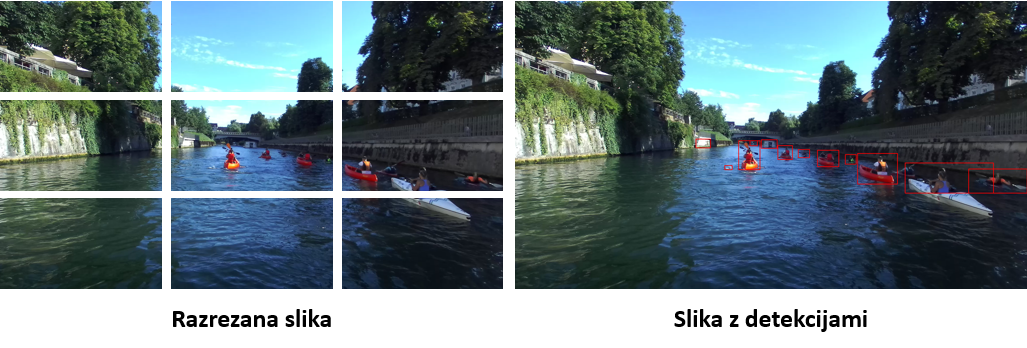
\includegraphics[width=0.5\textwidth]{Slike/Tiled_detection.PNG} % Vstavljanje slike
    \caption{Primer razrezane slike kot vhod in končna detekcija} % Napisan napis
    \label{fig:detekcija_po_delih} % Oznaka za referenciranje slike
\end{figure}

\subsection{Detekcija na termalnih slikah}
Detekcija ovir na termalnih slikah se od barvnih slik ni bistveni razlikovala. Podatki so bili enako obdelani kot ti za segmentacijo, torej pretvorjeni v tri kanalni 8-bitni zapis in razvrščeni v ustrezne mape. Za učenje so bili uporabljeni enaki parametri z razliko augmentacije slik, ki so bile enake kot v postopku učenja z barvnimi slikami vendar brez manipulacije baru, svetlost, nasičenosti itd. Ker gre za temperaturno sliko smo želeli to na posamezni oviri tudi ohraniti.

\begin{figure}[h!]
    \centering % Središčenje slike
    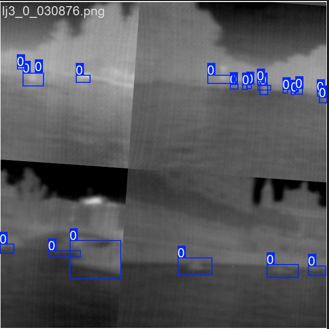
\includegraphics[width=0.35\textwidth]{Slike/augmented_image.PNG} % Vstavljanje slike
    \caption{Primer augmentirane slike} % Napisan napis
    \label{fig:augmented_image} % Oznaka za referenciranje slike
\end{figure}
%-------------------------------------------------------------------------

%%%%%%%%% REZULTATI
%-------------------------------------------------------------------------
\section{Rezultati}
Vse naučene modele se je nato testiralo. Za to se je uporabljalo le podatke podane v \texttt{test} datoteki, kateri niso bili uporabljeni v postopku učenja. Kot kvalitativno oceno se je pri segmentaciji uporabilo mIoU mero, pri detekciji pa mero f1. Vsak test je vse obdelane slike tudi lokalno shranil za vizualno preverjanje. Pri segmentaciji se je razrede na generiranih maskah pobarvalo v različne barve ter se nato tako obdelano masko z določeno prosojnostjo prekrilo čez vhodno sliko. Postopek detekcije je vse zaznane ovire shranil v obliki YOLO zapisa v datoteko. Te skupaj z vrednostjo verjetnosti se je nato narisalo na testne slike. V preizkusu z razrezanimi vhodnimi podatki so te ovire označene z drugo barvo in nimajo podatka o verjetnosti, saj so bile te naknadno narisane na osnovi več slik in podatkov.

\paragraph{Segmentacija barvnih slik\newline}
V prvem testu segmentacije se je teste izvajalo na dveh različnih arhitekturah a na enakih testnih podatkih. Ravno tako sta bili mreži naučeni na enakih učnih podatkih. Rezultati so podani v tabeli \ref{tab:rezultati_segmentacije_RGB}.

\begin{table}[h!]
    \begin{center}
        \begin{tabular}{|l|c|}
            \hline
                Arhitektura & mIoU \\
            \hline\hline
                U-Net & 0.757838 \\
                SegFormer & 0.772018 \\
            \hline
        \end{tabular}
    \end{center}
    \caption{Končna vrednost testa segmentacije barvnih slik}
    \label{tab:rezultati_segmentacije_RGB}
\end{table}

\begin{figure}[h!]
    \centering % Središčenje slike
    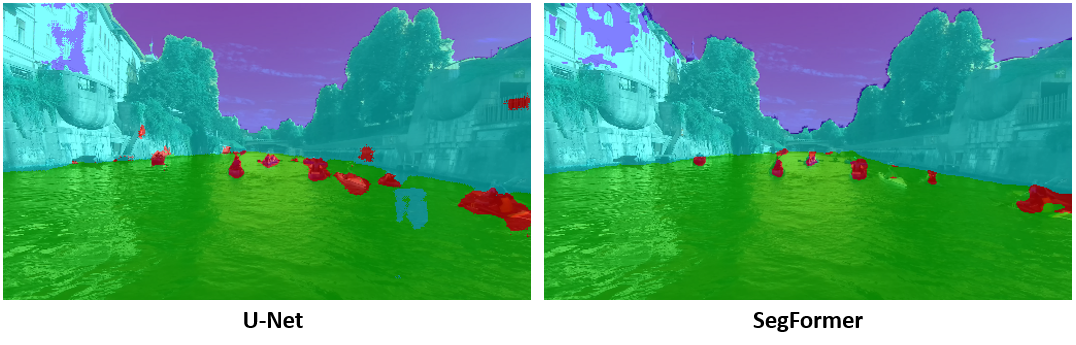
\includegraphics[width=0.5\textwidth]{Slike/unet_vs_segformer.PNG} % Vstavljanje slike
    \caption{Primerjava segmentacije mreže U-Net in SegFormer} % Napisan napis
    \label{fig:rezultati_segmentacije_RGB} % Oznaka za referenciranje slike
\end{figure}

Vrednosti nakazujejo, da sta si arhitekturi precej blizu v natančnosti segmentacije. Tako vizualno iz slike \ref{fig:rezultati_segmentacije_RGB} kot tudi iz ostalih slik je razvidno, da SegFormer naredi manj napačnih detekcij na okolici oz. bi lahko rekli, da so njegove napovedi manj pošumljene. Predvidevamo, da bi lahko kvaliteto segmentacije obeh še izboljšali z večjo količino učnih podatkov. To bi najverjetneje bistveno pripomoglo pri SegFormer-ju. Ker ta arhitektura temelji na osnovi transformerja, kateri so znano po tem, da zahtevalo velike količine podatkov bi to najverjetneje pomagalo tudi v tem primeru. Ravno tako osnoven model SegFormer-ja, ki je bil doučen ni bil najkompleksnejši od razpoložljivih.

\paragraph{Segmentacija termalnih slik\newline}
Kot omenjeno je bila segmentacija na termalnih slikah skoraj identična barvnim le z nekaj spremembami v nalagalniku podatkov. Ravno tako sta bili pri tem uporabljeni obe arhitekturi, torej U-Net in SegFormer. Rezultati so naslednji:

\begin{table}[h!]
    \begin{center}
        \begin{tabular}{|l|c|}
            \hline
                Arhitektura & mIoU \\
            \hline\hline
                U-Net & 0.681646 \\
                SegFormer & 0.793875 \\
            \hline
        \end{tabular}
    \end{center}
    \caption{Končna vrednost testa segmentacije termalnih slik}
    \label{tab:rezultati_segmentacije_thermal}
\end{table}

Tabela \ref{tab:rezultati_segmentacije_thermal} kaže na podobne rezultate kot segmentacija barvnih slih. Razlog za neenakomerne vrednosti rezultatov pa bi lahko najverjetneje pripisali resoluciji samih slik saj so te veliko manjše kot barvne in ob enem ne tako jasne. Na osnovi tega predvidevamo, da se je SegFormer bil sposoben naučiti kompleksnejših vzorcev. Če bi te želeli še izboljšati brez dodatnega učnega materiala bi lahko vsaj pri SegSormer-ju uporabili kompleksnejši osnovni model. Smiselno bi bilo tudi dodatno eksperimentiranje z augmentacijami. Kot je bilo opaženo v naših preizkusih vse ne vplivajo koristno na učenje.

\paragraph{Detekcija na barvnih slikah\newline}
Rezultati detekcije so presenetljivo slabši od pričakovanih. Kaj točno je vzrok temu ni jasno. Iz spodnjih tabel lahko vidimo, da zahtevnejši model te izboljša vendar vseeno je razlika majhna.

\begin{table}[h!]
    \begin{center}
        \begin{tabular}{|l|c|c|c|}
            \hline
                Mera & YOLO11-s & YOLO11-m & YOLO11-x \\
            \hline\hline
                Precision & 0.682 & 0.782 & 0.722 \\
                Recall & 0.410 & 0.449 & 0.477 \\
                F1 Score & 0.512 & 0.570 & 0.574 \\
            \hline
        \end{tabular}
    \end{center}
    \caption{Detekcije na barvnih slikah}
    \label{tab:rezultati_detekcija_cela_rgb}
\end{table}

Pri testih na razrezanih vhodnih slikah rahlo kršimo osnovno idejo same YOLO arhitekture. Bistvo te je, da v enem koraku obdela sliko in je ta kar se da hitra. Ker v tem primeru potrebujemo za obdelavo več korakov (vsako del slike posebej) in moramo nato vse dele sestavit v celoto, pa to ni več en korak. Vseeno smo test opravili zaradi zanimanja po kvaliteti detekcije. Rezultati so naslednji:

\begin{table}[h!]
    \begin{center}
        \begin{tabular}{|l|c|c|c|}
            \hline
                Mera & YOLO11-s & YOLO11-m & YOLO11-x \\
            \hline\hline
                Precision & 0.685 & 0.814 & 0.774 \\
                Recall & 0.540 & 0.561 & 0.560 \\
                F1 Score & 0.604 & 0.664 & 0.650 \\
            \hline
        \end{tabular}
    \end{center}
    \caption{Detekcije na razrezanih barvnih slikah}
    \label{tab:rezultati_detekcija_tile_rgb}
\end{table}

Kljub počasnejši inferenci so rezultati boljši. Detekcija ovir je boljša, sploh teh v daljavi, ki so na slikah manjše. Vseeno se pojavi več napačnih detekcij oz. dvojnih detekcij na eni oviri. Te so po večini na ovirah, ki se ob rezanju razdelijo v dve sliki, ali na kopnem kot so mostovi in dežniki. Obe napaki bi lahko z dodatno obdelavo pri združevanju delov slik v celoto odpravili, kar pa bi postopek še bolj upočasnilo.

\paragraph{Detekcija na termalnih slikah\newline}
Modeli uporabljeni za detekcijo ovir na vodni gladini na osnovi termalnih slik so bili enaki kot prej. Vrednosti testov so kot pričakovano nižje, saj so tudi slike težje razločne. Iz tabele \ref{tab:rezultati_detekcija_thermal} lahko vidimo da kompleksnejši model ne poda nobene večje prednosti pred enostavnejšimi. Na osnovi tega lahko sklepamo, da ta modaliteta sama po sebi ni najbolj primerna za detekcijo ovir. Smiselno bi jo bilo uporabiti v kombinaciji s katero drugo obliko vhodnih podatkov.

\begin{table}[h]
    \begin{center}
        \begin{tabular}{|l|c|c|c|}
            \hline
                Mera & YOLO11-s & YOLO11-m & YOLO11-x \\
            \hline\hline
                Precision & 0.500 & 0.562 & 0.578 \\
                Recall & 0.297 & 0.387 & 0.279 \\
                F1 Score & 0.373 & 0.380 & 0.376 \\
            \hline
        \end{tabular}
    \end{center}
    \caption{Detekcije na termalnih slikah}
    \label{tab:rezultati_detekcija_thermal}
\end{table}


%-------------------------------------------------------------------------
 
%%%%%%%%% ZAKLJUČEK
%-------------------------------------------------------------------------
\section{Zaključek}
V tem članku smo predstavili in primerjali različne pristope k semantični segmentaciji in detekciji ovir na vodni gladini, pri čemer smo uporabili barvne in termalne slike. Ugotovili smo, da tako klasični U-Net kot sodobnejši SegFormer zmoreta učinkovito segmentacijo, pri kateri je SegFormer pokazal nekoliko boljše rezultate, še posebej na termalnih slikah. Pri detekciji dinamičnih ovir se je YOLO11 izkazal za primernega, a rezultati kažejo, da je kakovost detekcije v veliki meri odvisna od kakovosti in količine učnih podatkov.

Med analizo podatkovne zbirke smo ugotovili, da ta ni bila le razmeroma majhna, ampak tudi ne najboljše anotirana, kar smo opazili pri vizualnem pregledu učnih vzorcev. Takšna omejitev je najbolj vplivala na rezultate segmentacije.

Za doseganje še boljših rezultatov bi predlagali razširitev in izboljšanje učne zbirke, bolj natančno anotacijo slik ter uporabo kompleksnejših arhitektur oz. naprednejših tehnik augmentacije podatkov. Poseben izziv ostaja zaznava manjših in redkejših ovir, kjer so globoke mreže še posebej občutljive na pomanjkanje unikatnih primerov. Ena od idej je tudi izpopolnitev postopka YOLO na razrezanih slikah, kljub temu, da krši osnovno idejo. Smiselno bi bilo dodati prostorsko kodiranje z idejo, da bi ta podatek mreži pomagal najti vzorec na kateri sliki pričakovati detekcije in kje ne.

Predstavljene ugotovitve lahko služijo kot izhodišče za nadaljnje delo na področju avtonomne plovbe in detekcije ovir na vodi, pri čemer bo izboljšanje in nadgradnja podatkovnih zbirk ključnega pomena za razvoj zanesljivejših modelov.

{\small
\bibliographystyle{ieee}
\bibliography{egbib}
}

\end{document}
